% Architecture figure. Compile separately: pdflatex architecture.tex
%
% Layout: a 3 x 3 grid of items. Each item is a large pictogram chip with its label set beside it,
% so the top and bottom of every chip stay free and each connection is a short straight arrow.
%   columns x = 1.0 / 7.0 / 13.0      rows y = 0 / -3.0 / -6.0      assets y = -8.2
%   row 1 (left to right) : stereo input -> frozen tokens -> transformer decoder
%   row 2 (parallel)      : the three heads the decoder drives, one per column
%   row 3 (left to right) : the geometric route and the fusion, aligned under the head that feeds it
% Column k of row 2 feeds column k of row 3, so those three links are straight verticals.
\documentclass[tikz,border=2pt]{standalone}
\usepackage{amsmath,amssymb,xcolor,graphicx,helvet}
\renewcommand{\familydefault}{\sfdefault}
% Notation (docs/07): keep consistent across text, figures and tables.
\newcommand{\PaperTitle}{Factored Interaction Fields: Learning Joint-Anchored Hand-Object Proximity Through Its Geometric Arguments}
\newcommand{\method}{FIF}
\newcommand{\field}{\mathbf{v}}
\newcommand{\joint}{\mathbf{p}}
\newcommand{\vtx}{\mathbf{q}}
\newcommand{\objpose}{\theta_o}
\newcommand{\Rot}{\mathbf{R}}
\newcommand{\trans}{\mathbf{t}}
\newcommand{\mesh}{\mathcal{Q}}
\newcommand{\ade}{\mathrm{ADE}}
\newcommand{\mm}{\,\mathrm{mm}}
\newcommand{\ie}{i.e.}
\newcommand{\eg}{e.g.}

\usetikzlibrary{arrows.meta,calc,backgrounds}

\definecolor{cInk}{HTML}{2F343B}
\definecolor{cSlate}{HTML}{6F7885}\definecolor{cSlateF}{HTML}{EFF1F4}
\definecolor{cPlum}{HTML}{6B4E8E}\definecolor{cPlumF}{HTML}{F1ECF7}
\definecolor{cTeal}{HTML}{0F7B84}\definecolor{cTealF}{HTML}{E2F0F2}
\definecolor{cAmber}{HTML}{B8781A}\definecolor{cAmberF}{HTML}{FBF1DE}
\definecolor{cLoss}{HTML}{A32B2B}
\newcommand{\m}[1]{\mbox{$#1$}}

\begin{document}
\begin{tikzpicture}[x=1cm,y=1cm,
  chip/.style={draw, rounded corners=2.2pt, minimum width=16mm, minimum height=16mm, line width=0.6pt, inner sep=0},
  cslate/.style={chip, draw=cSlate, fill=cSlateF},
  cplum/.style={chip, draw=cPlum, fill=cPlumF},
  cteal/.style={chip, draw=cTeal, fill=cTealF},
  camber/.style={chip, draw=cAmber, fill=cAmberF},
  photo/.style={inner sep=0, draw=cSlate!65, line width=0.4pt},
  arr/.style={-{Latex[length=2.1mm,width=1.7mm]}, line width=0.65pt, draw=cInk!80},
  wire/.style={line width=0.65pt, draw=cInk!80},
  capt/.style={font=\scriptsize, text=cInk!78, align=left, inner sep=0},
  tag/.style={font=\scriptsize, text=cInk!62, inner sep=1.5pt},
  ico/.style={x=1mm, y=1mm, sharp corners, line cap=round, line join=round, line width=0.55pt},
]
% label beside a chip: bold name, then one small descriptive line
\def\lab#1#2#3{\node[anchor=west, text width=29mm, align=left, inner sep=0, font=\footnotesize,
  text=cInk] at #1 {\textbf{#2}\\[0.5mm]{\scriptsize\textcolor{cInk!78}{#3}}};}

% ============================================================ row 1: perception (y = 0)
\node[photo] (imgB) at (1.32,-0.22) {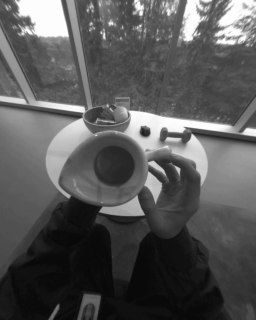
\includegraphics[width=10mm]{thumb_in1.png}};
\node[photo] (imgA) at (0.78,0.22) {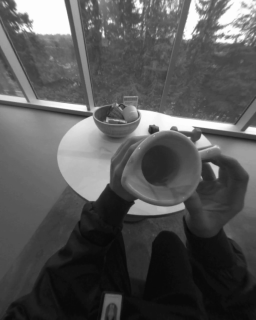
\includegraphics[width=10mm]{thumb_in0.png}};
\lab{(2.05,0)}{stereo input}{two synchronised headset views, $1024{\times}1280$}

\node[cslate] (enc) at (7.0,0) {};
\begin{scope}[ico, shift={(enc.center)}]
  \foreach \i in {0,1,2}{\foreach \j in {0,1,2}{%
    \draw[cSlate!75, fill=cSlate!20] (-1.0+\i*2.6,-4.0+\j*2.6) rectangle ++(2.3,2.3);}}
  \foreach \p in {(-2.0,-1.9),(-2.4,-0.2),(-1.5,-3.5)}{\draw[cPlum!85, line width=0.4pt] (-5.0,-3.6) -- \p;}
  \fill[cPlum] (-5.0,-3.6) circle (0.75);
  \foreach \a in {0,60,120}{\draw[cSlate, line width=0.6pt] (-4.6,4.4) +(\a:1.75) -- +({\a+180}:1.75);}
  \fill[cSlate] (-4.6,4.4) circle (0.4);
\end{scope}
\lab{(8.05,0)}{frozen tokens}{DINOv3 ViT-B/16 patches of both views, each tagged with its Pl\"ucker ray}

\node[cplum] (dec) at (13.0,0) {};
\begin{scope}[ico, shift={(dec.center)}]
  \foreach \a/\b in {-4.5/-4.8,-4.5/-2.4,-1.5/-2.4,-1.5/0,1.5/0,1.5/2.4,4.5/2.4,4.5/4.8,-1.5/-4.8,4.5/0}{%
    \draw[cPlum!45, line width=0.35pt] (\a,3.7) -- (\b,-3.7);}
  \foreach \x in {-4.5,-1.5,1.5,4.5}{\fill[cPlum] (\x,4.2) circle (0.85);}
  \foreach \x in {-4.8,-2.4,0,2.4,4.8}{\draw[cPlum, fill=white, line width=0.45pt] (\x-0.7,-4.9) rectangle ++(1.4,1.4);}
\end{scope}
\lab{(14.05,0)}{transformer decoder}{$L{=}6$ layers; 42 joint and 16 object queries}

\draw[arr] (5.15,0) -- (6.20,0);
\draw[arr] (11.15,0) -- (12.20,0);

% ============================================================ row 2: the three heads (y = -3.0)
\node[cplum] (hobj) at (1.0,-3.0) {};
\begin{scope}[ico, shift={(hobj.center)}]
  \draw[cPlum, fill=cPlum!12] (90:4.3) -- (162:4.3) -- (234:4.3) -- (306:4.3) -- (18:4.3) -- cycle;
  \foreach \a in {90,162,234,306,18}{\draw[cPlum!70, line width=0.4pt] (0,0) -- (\a:4.3);}
  \foreach \a in {90,162,234,306,18}{\fill[cPlum] (\a:4.3) circle (0.95);}
  \fill[cPlum!55] (0,0) circle (0.7);
\end{scope}
\lab{(2.05,-3.0)}{object control-point head}{control points $\hat{\mathbf{c}}_n$ with confidences $w_n$}

\node[cplum] (hjnt) at (7.0,-3.0) {};
\begin{scope}[ico, shift={(hjnt.center)}]
  \foreach \c in {{(-3.6,-2.6),(-4.9,-0.7),(-5.5,1.0)},{(-1.8,-1.0),(-2.1,1.4),(-2.3,3.6)},%
                  {(0,-0.8),(0,1.8),(0,4.4)},{(1.8,-1.0),(2.1,1.4),(2.3,3.6)},{(3.4,-1.8),(4.0,0.3),(4.3,2.3)}}{%
    \draw[cPlum, line width=0.5pt] (0,-4.8) \foreach \p in \c {-- \p};
    \foreach \p in \c {\fill[cPlum] \p circle (0.6);}}
  \fill[cPlum] (0,-4.8) circle (0.8);
\end{scope}
\lab{(8.05,-3.0)}{joint head}{camera-frame hand joints $\hat{\joint}_{h,j}$, in millimetres}

\node[cplum] (hdir) at (13.0,-3.0) {};
\begin{scope}[ico, shift={(hdir.center)}]
  \draw[cPlum!55, dash pattern=on 0.7mm off 0.45mm, line width=0.45pt] (2.4,2.4) circle (2.4);
  \draw[cPlum, -{Latex[length=1.9mm,width=1.5mm]}, line width=0.8pt] (-4.2,-4.2) -- (2.3,2.3);
  \fill[cPlum] (-4.2,-4.2) circle (0.9);
\end{scope}
\lab{(14.05,-3.0)}{direct head}{the field \m{\field^{\rm dir}} and its \mbox{log-scale} \m{s^{\rm dir}}}

% query bus: one drop from the decoder, one channel, three taps
\draw[wire] (dec.south) -- (13.0,-1.55);
\draw[wire] (1.0,-1.55) -- (13.0,-1.55);
\foreach \x in {1.0,7.0,13.0}{\draw[arr] (\x,-1.55) -- (\x,-2.20);}
\node[tag, anchor=south] at (10.2,-1.50) {refined queries};

% ============================================================ row 3: geometry and fusion (y = -6.0)
\node[cteal] (proc) at (1.0,-6.0) {};
\begin{scope}[ico, shift={(proc.center)}]
  \draw[cTeal!55, densely dashed, line width=0.45pt] (-5.0,-4.4) -- (-1.0,-5.2) -- (-2.6,-1.2) -- cycle;
  \foreach \p in {(-5.0,-4.4),(-1.0,-5.2),(-2.6,-1.2)}{\draw[cTeal!75, fill=white, line width=0.45pt] \p circle (0.75);}
  \draw[cTeal] (1.1,0.6) -- (5.2,1.5) -- (2.4,4.8) -- cycle;
  \foreach \p in {(1.1,0.6),(5.2,1.5),(2.4,4.8)}{\fill[cTeal] \p circle (0.8);}
  \draw[cTeal, -{Latex[length=1.7mm,width=1.4mm]}, line width=0.6pt] (-2.4,0.6) to[bend left=32] (0.5,3.4);
\end{scope}
\lab{(2.05,-6.0)}{weighted Procrustes}{object pose $(\hat{\Rot}_o,\hat{\trans}_o)$ in closed form, differentiable}

\node[cteal] (snn) at (7.0,-6.0) {};
\begin{scope}[ico, shift={(snn.center)}]
  \draw[cTeal, line width=0.65pt] (-5.5,1.4) -- (-2.5,3.6) -- (0.4,1.1) -- (3.4,3.3) -- (5.5,0.9);
  \draw[cTeal!45, dash pattern=on 0.7mm off 0.45mm, line width=0.45pt] (0.4,1.1) circle (2.3);
  \foreach \p in {(-5.5,1.4),(-2.5,3.6),(0.4,1.1),(3.4,3.3),(5.5,0.9)}{\fill[cTeal] \p circle (0.7);}
  \draw[cTeal, -{Latex[length=1.9mm,width=1.5mm]}, line width=0.8pt] (-1.4,-4.6) -- (0.25,-0.3);
  \fill[cPlum] (-1.4,-4.6) circle (0.9);
\end{scope}
\lab{(8.05,-6.0)}{soft nearest vertex}{the geometric field $\field^{\rm geo}$, evaluated on the posed mesh}

\node[camber] (fus) at (13.0,-6.0) {};
\begin{scope}[ico, shift={(fus.center)}]
  \draw[cInk!25, line width=0.4pt] (-5.4,-4.2) -- (5.4,-4.2);
  \draw[cTeal, line width=0.65pt] plot[domain=-5.4:5.4,samples=44,smooth] (\x,{-4.2+3.4*exp(-pow(\x-1.9,2)/9.0)});
  \draw[cPlum, line width=0.65pt] plot[domain=-5.4:5.4,samples=44,smooth] (\x,{-4.2+8.2*exp(-pow(\x+1.6,2)/1.6)});
  \draw[cAmber, line width=0.8pt] (-1.05,-4.6) -- (-1.05,4.6);
  \fill[cAmber] (-1.05,4.6) circle (0.65);
\end{scope}
\lab{(14.05,-6.0)}{precision-weighted fusion}{per-joint weights \m{\lambda^{k}=e^{-2s^{k}}} from the predicted scales}

% row 2 feeds row 3, one straight vertical per column
\foreach \x in {1.0,7.0,13.0}{\draw[arr] (\x,-3.80) -- (\x,-5.20);}
% the geometric route, left to right
\draw[arr] (5.15,-6.0) -- (6.20,-6.0);
\draw[arr] (11.15,-6.0) -- (12.20,-6.0);

% ============================================================ given asset and output (y = -8.2)
\node[cslate, minimum width=14mm, minimum height=14mm] (meshc) at (1.0,-8.2) {};
\node[inner sep=0] at (meshc.center) {\includegraphics[width=12mm]{thumb_mesh.png}};
\draw[arr] (1.0,-7.50) -- (1.0,-6.80);
\node[capt, anchor=west, text width=29mm] at (2.05,-8.2)
  {\textbf{canonical mesh}, given with the object alias: 16 control points $\mathbf{c}_n$, 1{,}024 vertices $\vtx_m$};

\node[photo] (out) at (13.0,-8.2) {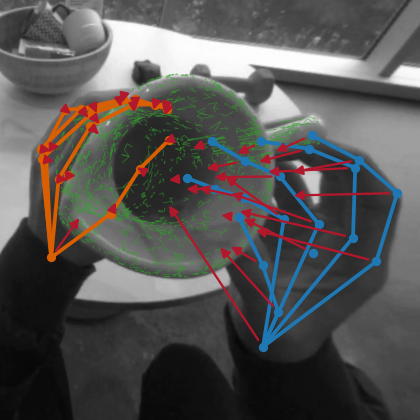
\includegraphics[width=16mm]{thumb_out.png}};
\draw[arr] (13.0,-6.80) -- (13.0,-7.50);
\node[capt, anchor=west, text width=29mm] at (14.05,-8.2)
  {\textbf{predicted field}, rotated into the world frame: $2{\times}21{\times}3$ values in mm};

% training losses
\node[anchor=north, text width=46mm, align=center, font=\scriptsize, text=cLoss] at (7.0,-7.40)
  {\textbf{training:} endpoint error of the fused field, a Gaussian NLL per head, and auxiliary $\mathcal{L}_{\rm joint}$, $\mathcal{L}_{\rm obj}$, $\mathcal{L}_{\rm vis}$, $\mathcal{L}_{\rm pres}$ on the heads};

% ============================================================ colour key
\begin{scope}[shift={(0.25,1.45)}]
  \node[cslate, minimum width=5mm, minimum height=2.6mm] (k1) at (0,0) {};
  \node[tag, anchor=west] (t1) at (0.32,0) {frozen or given};
  \node[cplum, minimum width=5mm, minimum height=2.6mm] (k2) at ($(t1.east)+(0.5,0)$) {};
  \node[tag, anchor=west] (t2) at ($(k2.east)+(0.08,0)$) {trained};
  \node[cteal, minimum width=5mm, minimum height=2.6mm] (k3) at ($(t2.east)+(0.5,0)$) {};
  \node[tag, anchor=west] (t3) at ($(k3.east)+(0.08,0)$) {differentiable geometry, no parameters};
  \node[camber, minimum width=5mm, minimum height=2.6mm] (k4) at ($(t3.east)+(0.5,0)$) {};
  \node[tag, anchor=west] (t4) at ($(k4.east)+(0.08,0)$) {fusion};
\end{scope}
\end{tikzpicture}
\end{document}
